\chapter{Entropic forces and Cosolute Flows}
\label{chap:entropic_force}

\section{Experimental Motivation}
When considering the structural dynamics and functionality of macromolecules, the effective volume of the surrounding environment is a  critical factor. Conditions in typical cellular environments are often filled with other molecules whose size is on the same order as macromolecules. As the environment gets crowded, the mutual impenetrability of the particles gives rise to excluded volume effects and has significant consequences for protein stability and folding rate,\cite{minton_can_2006, ping_depletion_2006, rosgen_protein_2005, pincus_crowding_2009, cheung_effects_2007, cheung_molecular_2005, stagg_molecular_2007, minton_models_2005, sasahara_effect_2003} chaperonin action\cite{zhou_protein_2004} and amyloid fibril formation.\cite{kinoshita_ordered_2004} Crowded environments may also enhance the rate of protein aggregation \cite{ellis_protein_2006}. A comprehensive review of macromolecular crowding can be found in \cite{huan-xiang_zhou_macromolecular_2008}. 

Along this line, two recent experiments are the motivation for the present work. The first is the single-molecule measurement of the mechanical force required to unfold a protein molecule (ubiquitin) using atomic force microscopy (AFM). It was found that at fixed pulling speed the unfolding force increased progressively as more crowders are added.\cite{yuan_effects_2008} Our model here assumes the globular protein is mainly spherical in shape and when stretched under the AFM, elliptic. Furthermore, while the protein molecules are under stretch they are not free to move. Therefore, for simplicity we consider the limiting case that the stretched protein is an infinitely heavy hard ellipse which is stationary under collisions with the crowder molecules. In this paper, we have restricted ourselves to a 2D system. 

%********************
The effect caused by the addition of cosolutes observed in these experiments is the result of the interplay of the entropic effect of the macromolecule, cosolute and water. Since the cosolutes added are typically hydrophilic, their addition causes an increase in the total packing fraction of the aqueous solution, leading to a stronger crowding effect.\cite{akiyama_remarkable_2006} Nevertheless, a single-component system is still a useful tool to elucidate the physical nature of the entropic excluded volume effect. Our work considers the dynamics of a large heavy solute immersed in a bath of hard-spheres to model these observations of crowding-enhanced protein stability.

%********************

Another related experiment showed that a crowded environment can induce shape change in protein molecules (Borrelia burgdorferi VIsE) from a non-spherical native structure to a more compact non-native spherical structure.\cite{homouz_crowded_2008} Associated with this shape change, the function of protein may change as a result. An interesting question to ask is then: Can a non-spherical molecule experience an intra-molecular attraction, somewhat similar to the role of  surface tension, change its shape into a spherical one due to the presence of crowders?  An objective of the present article is to try to answer this question by studying the collision dynamics between hard-disc crowders and a hard ellipse. 

The first study of excluded-volume effects, also known as the depletion force, was originally derived by Asakura and Oosawa\cite{asakura_interaction_1958} for hard spheres. AO theory assumes that the density of the crowders is uniform for all permissible volumes and the excluded volume is simply the volume of the offset shape. The offset for a single convex particle is defined as the surface extended some distance normally from the surface. The excluded volume modifies the partition function by restricting the space available to the particles. The closer two particles are, the more volume is available to the remaining crowders and hence a stronger depletion force. By simple geometric arguments, AO theory gives an attractive interaction for hard discs that scales monotonically with the inter-particle separation. Essentially this is the zeroth-order term in integral equation theories based on statistical mechanics. The true spatial distribution is dependent on pair-wise correlations, which themselves are dependent on three-point correlations, etc. To move beyond AO theory requires detailed knowledge of these higher-order correlation functions. The Ornstein-Zernike equation, an open equation that gives the exact distribution function, can be solved analytically under proper closure relations such as the Percus-Yevick (PY) relation for hard spheres,\cite{wertheim_exact_1963} and hard ellipses.\cite{ward_structure_1988} The PY closure gives good results for low size asymmetry and packing fractions, outside this domain it can lead to pathological results for the density profiles. An alternative closure relation, hypernetted-chain (HNC) \cite{van_leeuwen_new_1959} has been shown to give results more consistent with numerical simulations.\cite{kinoshita_interaction_1996}

This tendency of hard-disc or hard-sphere objects to feel an inter-particle entropic force has previously been observed in physical experiments,\cite{crocker_entropic_1999, ohshima_direct_1997} theoretical predictions,\cite{tehver_depletion_1999, mao_depletion_1995} and computer simulations.\cite{biben_depletion_1996} The impenetrability of the molecules, a nonspecific steric repulsion, forms the basis of this entropic force. The loss of entropy between the two particles is overcome by the gain in the entropy of the remaining particles. 

An interesting effect resulting from the theory of depletion force is the tendency for particles to move along surfaces of decreasing curvature for convex surfaces (and equivalently, increasing curvature for concave surfaces). The depletion zone a crowder makes at contact is greater for a flatter surface, hence the particle should, on average, feel a force in this direction. Studies of various geometries using integral theories\cite{kinoshita_interaction_2004, kinoshita_spatial_2002} and density functional theory\cite{roth_depletion_1999, roth_depletion_2000} have confirmed this fact. This has been experimentally observed for colloidal particles that feel repulsion near a sharp edge.\cite{dinsmore_entropic_1996} Manipulation of colloidal structures has an obvious appeal, but typically these studies focus on the density profiles and not the resulting velocity patterns that arise from the entropic interaction. In this chapter we provide evidence of the entropic flows arising from hard potential surfaces.

If a crowder tends to move along regions of decreasing depletion areas, one should observe a flow of entropic origin surrounding non-uniformly curved surfaces. If we vary the geometry of a fixed macromolecule, say from a circle to an ellipse, it is possible to change these density profiles and resulting flows.  We investigate this effect by varying the shape of the ellipse as well as the different packing fractions and the relative size of the crowders. 

In a biological system, water cannot be regarded as an inert background.\cite{kinoshita_roles_2006} The presence of a solute generates an excluded volume not only for the other solutes but also for water molecules. To exclusively investigate the entropic excluded-volume effect, water molecules can also be modeled as hard spheres. In a strict sense, ``crowders'' should be treated as a multi-component system.\cite{akiyama_remarkable_2006} However, considering water molecules explicitly in a multi-component system would greatly increase the complexity of the computation. We shall therefore focus on the depletion effects of one-component crowders on a non-spherical body in the present study.

%For a biological system, the solvent water molecules have unique properties, related to its dipole moment, the dielectric constant and its tendency to form hydrogen-bonded clusters. In the present study of the excluded volume effects between hard bodies, we do not take solvent into explicit consideration. If we do, the net excluded volume effect can be significantly greater, as shown by Akiyama \cite{akiyama_remarkable_2006} \emph{et al.} However, considering solvent molecules explicitly in a multicomponent system would greatly increase the complexity of the computation. We shall therefore focus exclusively on the depletion effects of crowders on a non-spherical body in the present study.

%The resulting microscopic structure of the solution certainly plays a role in determining the system properties. In a strict sense, one should consider both the crowders and the solvent explicitly as a multi-component system. Unlike true colloidal suspensions however, there are no biological systems that can be treated as hard-body models in real experiments \cite{kinoshita_roles_2006}. We therefore investigate the entropic effect exclusively in the present model by employing a hard-body potential of a large macromolecule immersed in a single-component solution.

This chapter covers the computational method first, detailing the design parameters and the implementation of the discrete molecular dynamics. This is followed by the results of the simulations, along with a quantitative analysis on the boundary condition itself. The final section outlines the importance of the velocity fields along with their connections to the original motivating experiments.

\section{Computer simulations}


\subsection{Simulation design}

In the present work, we examine the flow of hard-discs around a hard ellipse fixed at the origin. The entire simulation is done using discrete molecular dynamics (DMD) as each potential collision can be predicted analytically. Initially the time of first collision for all disc pairs is found, along with the interaction against the interior boundary condition. This list is chronologically ordered and the simulation is integrated to the first collision. The collision is handled, conserving energy and impact angle and the collisions for the interacting discs are recalculated with the new velocity vectors. 

Calculating a collision between hard-discs is trivial. Given two velocity vectors, initial positions and radii of $r_a, r_b$, the discs first intersect when the positions are exactly a distance of $r_a + r_b$ apart. The exact time of collision can be reduced to a quadratic equation, whose discriminant is zero when the discs do not collide.

The collision of a disc with any other closed surface is, in general, a difficult problem to solve analytically. If the shape is convex, then the disc can intersect with the surface at most four times. The first point of collision can be found by setting the discriminant to zero, corresponding to a multiplicity of the roots, or identically the first point of collision. The collision can then be found by plugging this solution into the general solution of the fourth order intersection polynomial. This collision can also be visualized as the first point of intersection between a line and the offset of the convex shape. If the offset has a simple form, the problem simplifies greatly. For a disc, the offset \textit{is} another disc, whose collision is trivial. For an ellipse the offset shape is complicated, often requiring an iterative solution. The problem of two translating, rotating ellipses can be solved however, by reducing the problem to the roots of a simpler eighth-order polynomial.\cite{yi-king_choi_continuous_2006}

\subsection{Boundary conditions}
Using a dimensionless unit of length $L$ the system of interest is enclosed in a two-dimensional square box centered at the origin. The side length was $2L$ using periodic boundary conditions. Each hard-disc was given an initial velocity vector in a random direction whose magnitude was drawn from Gaussian distribution. The interior boundary condition was an ellipse, whose offset was defined as the surface extended normally a distance $r$. The ellipse defined with axes $E_a,E_b$ was parametrized as
%
\begin{equation}
\vec Q(\phi) = \begin{bmatrix}
	E_a \cos \phi \\
	E_b \sin \phi \\ 
\end{bmatrix} \\
\end{equation}

The first point of contact made by a hard-disc of radius $r$ with the ellipse is the intersection of its velocity ray with the ellipse offset
%
\begin{equation}
\vec Q_{\textit{offset}} = \vec Q + r\hat N
\end{equation}
%
Where $\hat N$ is the outward unit vector normal to the surface. The parametric form for the offset shape is thus
%
\begin{equation}
\vec Q(\phi) = \begin{bmatrix}
	E_a \cos \phi  + g r E_b \cos \phi\\
	E_b \sin \phi  + g r E_a \sin \phi\\
\end{bmatrix} \end{equation}
%
where $g={((E_b \cos \phi)^2 + (E_a \sin \phi)^2)}^{-1/2}$.

\section{Results}

The crowders consisted of a fixed number $N=50$ of homogeneous hard-discs whose radius varied according to packing fraction values of $\Pi=0.10$ to $\Pi=0.30$ with fixed aspect ratio of $k \equiv E_a/E_b$. For comparison, cellular interiors show approximately 20-30\% volume occupation by macromolecules.\cite{ellis_macromolecular_2001} 

Statistical averages of the velocity and density fields were taken by dividing the system into $150^2$ square cells. Snapshots of the fields were taken after $1/5$ of the total simulation time to allow for an initial thermalizing of the system. The resulting density patterns shown in FIG. \ref{fig:density_plot} are complex, but similar to other studies of hard-solutes near boundary conditions. As an example, consider in FIG. \ref{fig:radial_plot} the density distributions plotted along the major and minor axes. Each curve is zero inside the depletion zone, then it exhibits characteristic oscillations on the length scale of the crowder diameter. The reason for this is well known, the crowder statistically prefers to form shells around immobile barriers. It is also clear from the earlier discussion that the density on-contact should be larger for the minor (flatter) axis of the ellipse, as the depletion force there is greater.

\begin{figure}
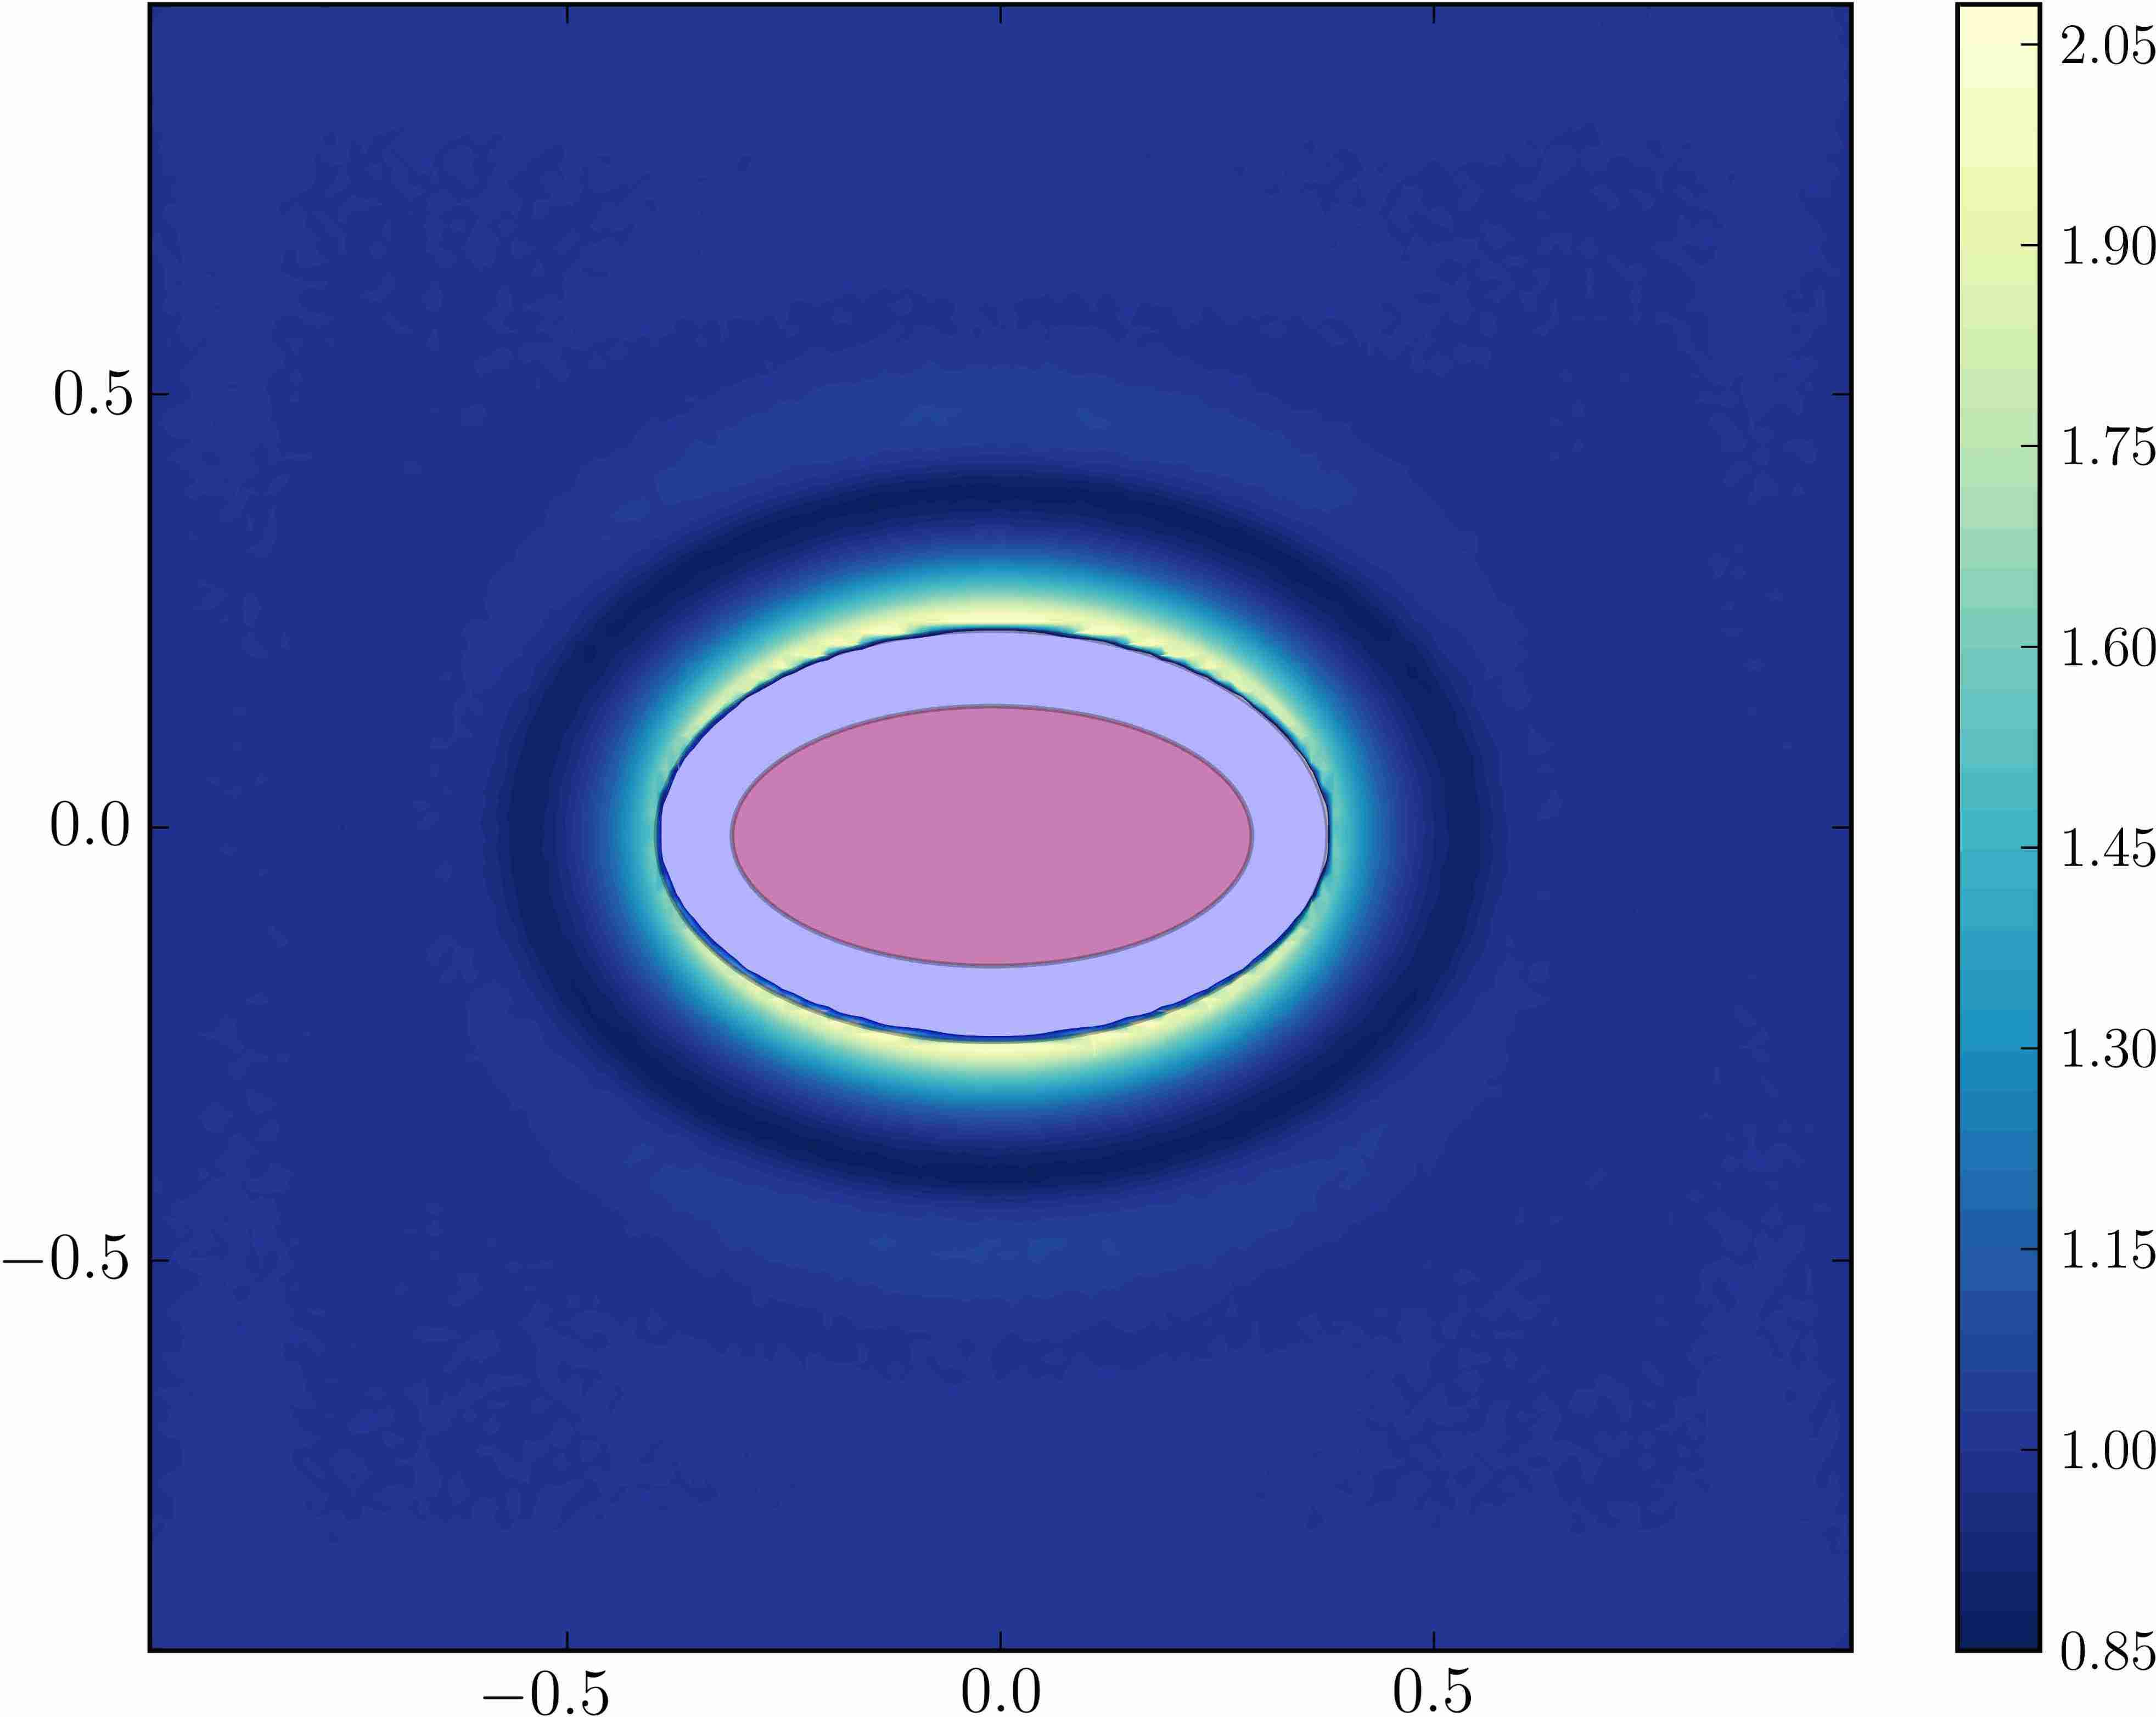
\includegraphics[width=\figurewidthSINGLE]{entropic_flow_paper/FIG1_EDIT.jpg}
\caption{Contours of averaged density profiles for an aspect ratio $k=2.0$, packing fraction $\Pi=0.30$, and relative crowder radius $r_c/L=0.04370$. The density has been normalized such that the bulk density is unity. Both the hard-ellipse and an approximation of the depletion zone are shown schematically.}
\label{fig:density_plot}
\end{figure}

\begin{figure}
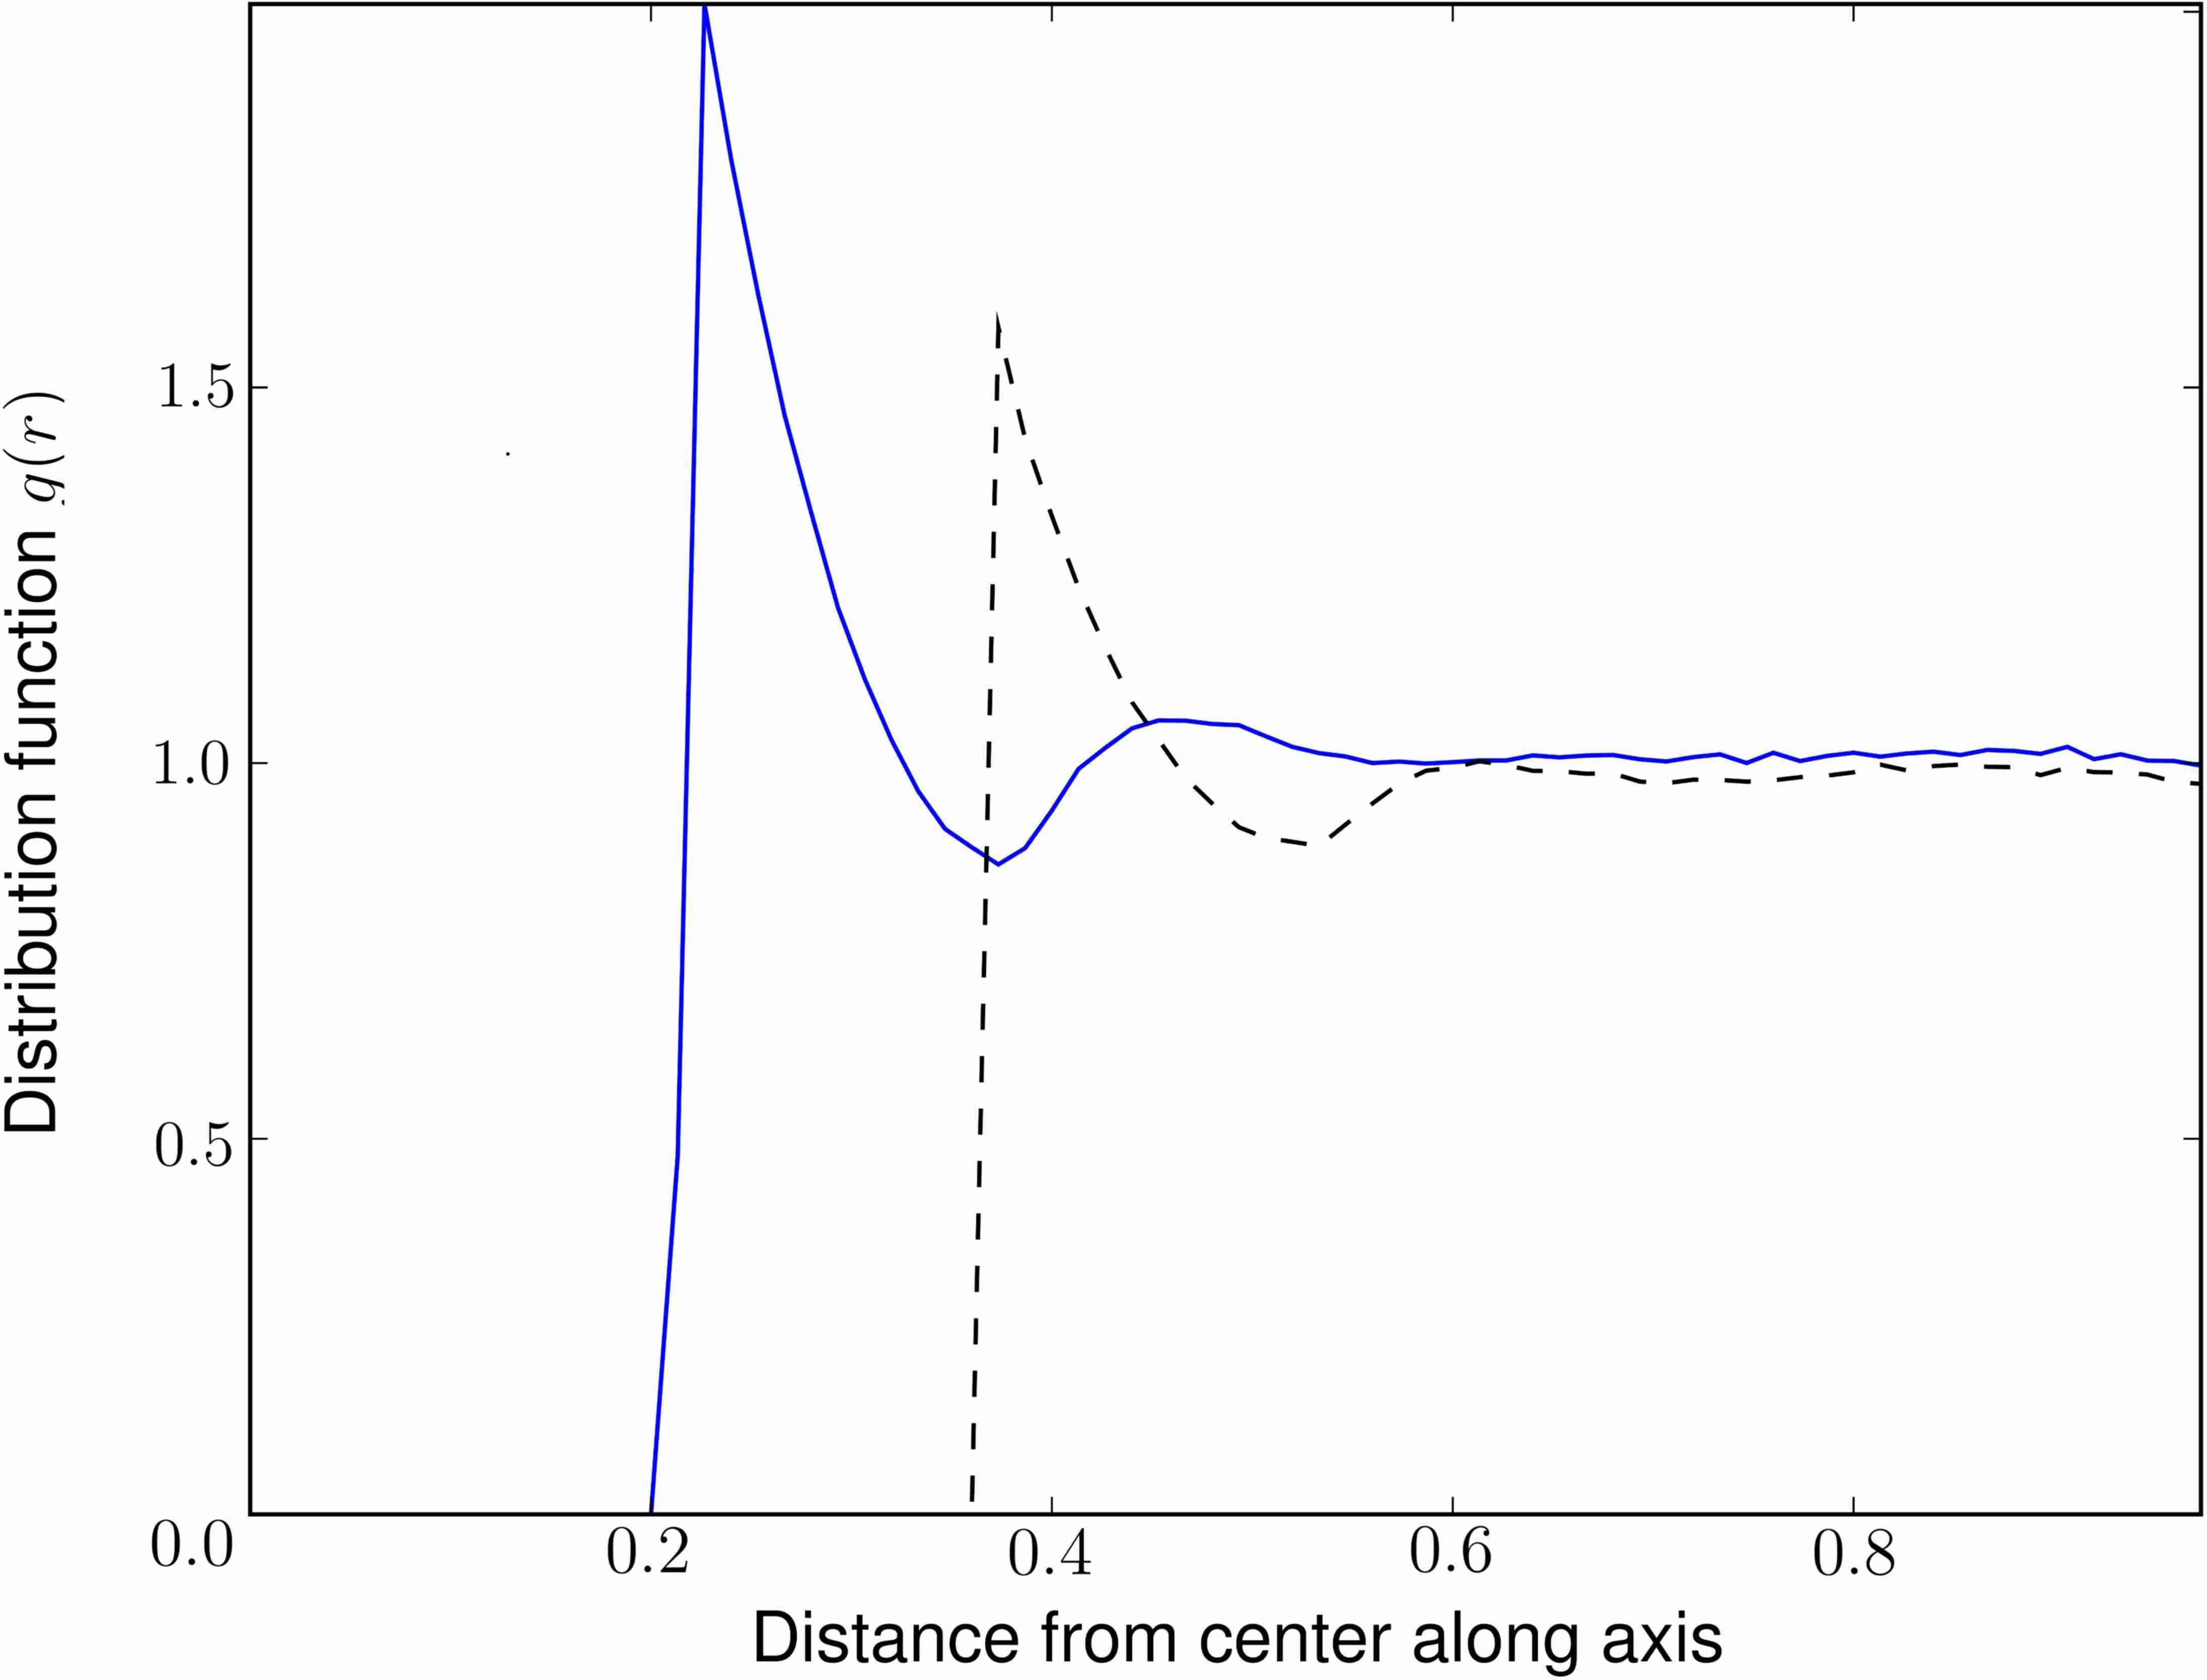
\includegraphics[width=\figurewidthSINGLE]{entropic_flow_paper/FIG2_EDIT.jpg}
\caption{Generalized distribution function along each elliptical axis for the parameters aspect ratio $k=2.0$, packing fraction $\Pi=0.30$, and relative crowder radius $r_c/L=0.04370$. The distribution function $g(r)$, is a measure of the average density at a point, normalized to one at the bulk density. The position of the function is to be taken from the origin along the specified axis, with the distance in units of $L$. The blue (solid) and black (dashed) curves denote the values along the minor and major axis respectively. The density on-contact is significantly greater at the minor axis of the ellipse. The curves exhibits characteristic oscillations at precisely the crowder diameter. }
\label{fig:radial_plot}
\end{figure}

Interestingly, when we plot the time-averaged velocity field near the hard ellipse the field exhibits four vortices. Since the system has four-fold symmetry (up to a sign change in the curl of the velocity field), we show only a portion of the upper quadrant of the velocity in FIG. \ref{fig:velocity_plot}. The velocity field clearly exhibits a single vortex, one that remains stable in both size and location for the duration of the simulation. The net angular momentum of the system is still zero as each vortex has a counter-rotating partner, but the distribution of the momentum has been partitioned along the quadrant lines. This is an initially surprising result, as such flows are usually caused by a thermal gradient, advective field or other potential. The entropic flows observed here are completely the result of treating the ellipse as a hard boundary (rather than a free particle), which serves to redistribute the angular momentum of the system. This is discussed further in next section. The exterior periodic boundary conditions serve to enclose the flow. It is unknown if the flows obtained are still valid in an infinite bath ($L \rightarrow \infty$). The deviation from uniformity of both the density and velocity fields occurs whenever $k \neq 1$. As the the aspect ratio approaches unity ($k \rightarrow 1$) the pattern generation takes longer to develop implying that there are no observed phase transitions.

\begin{figure}
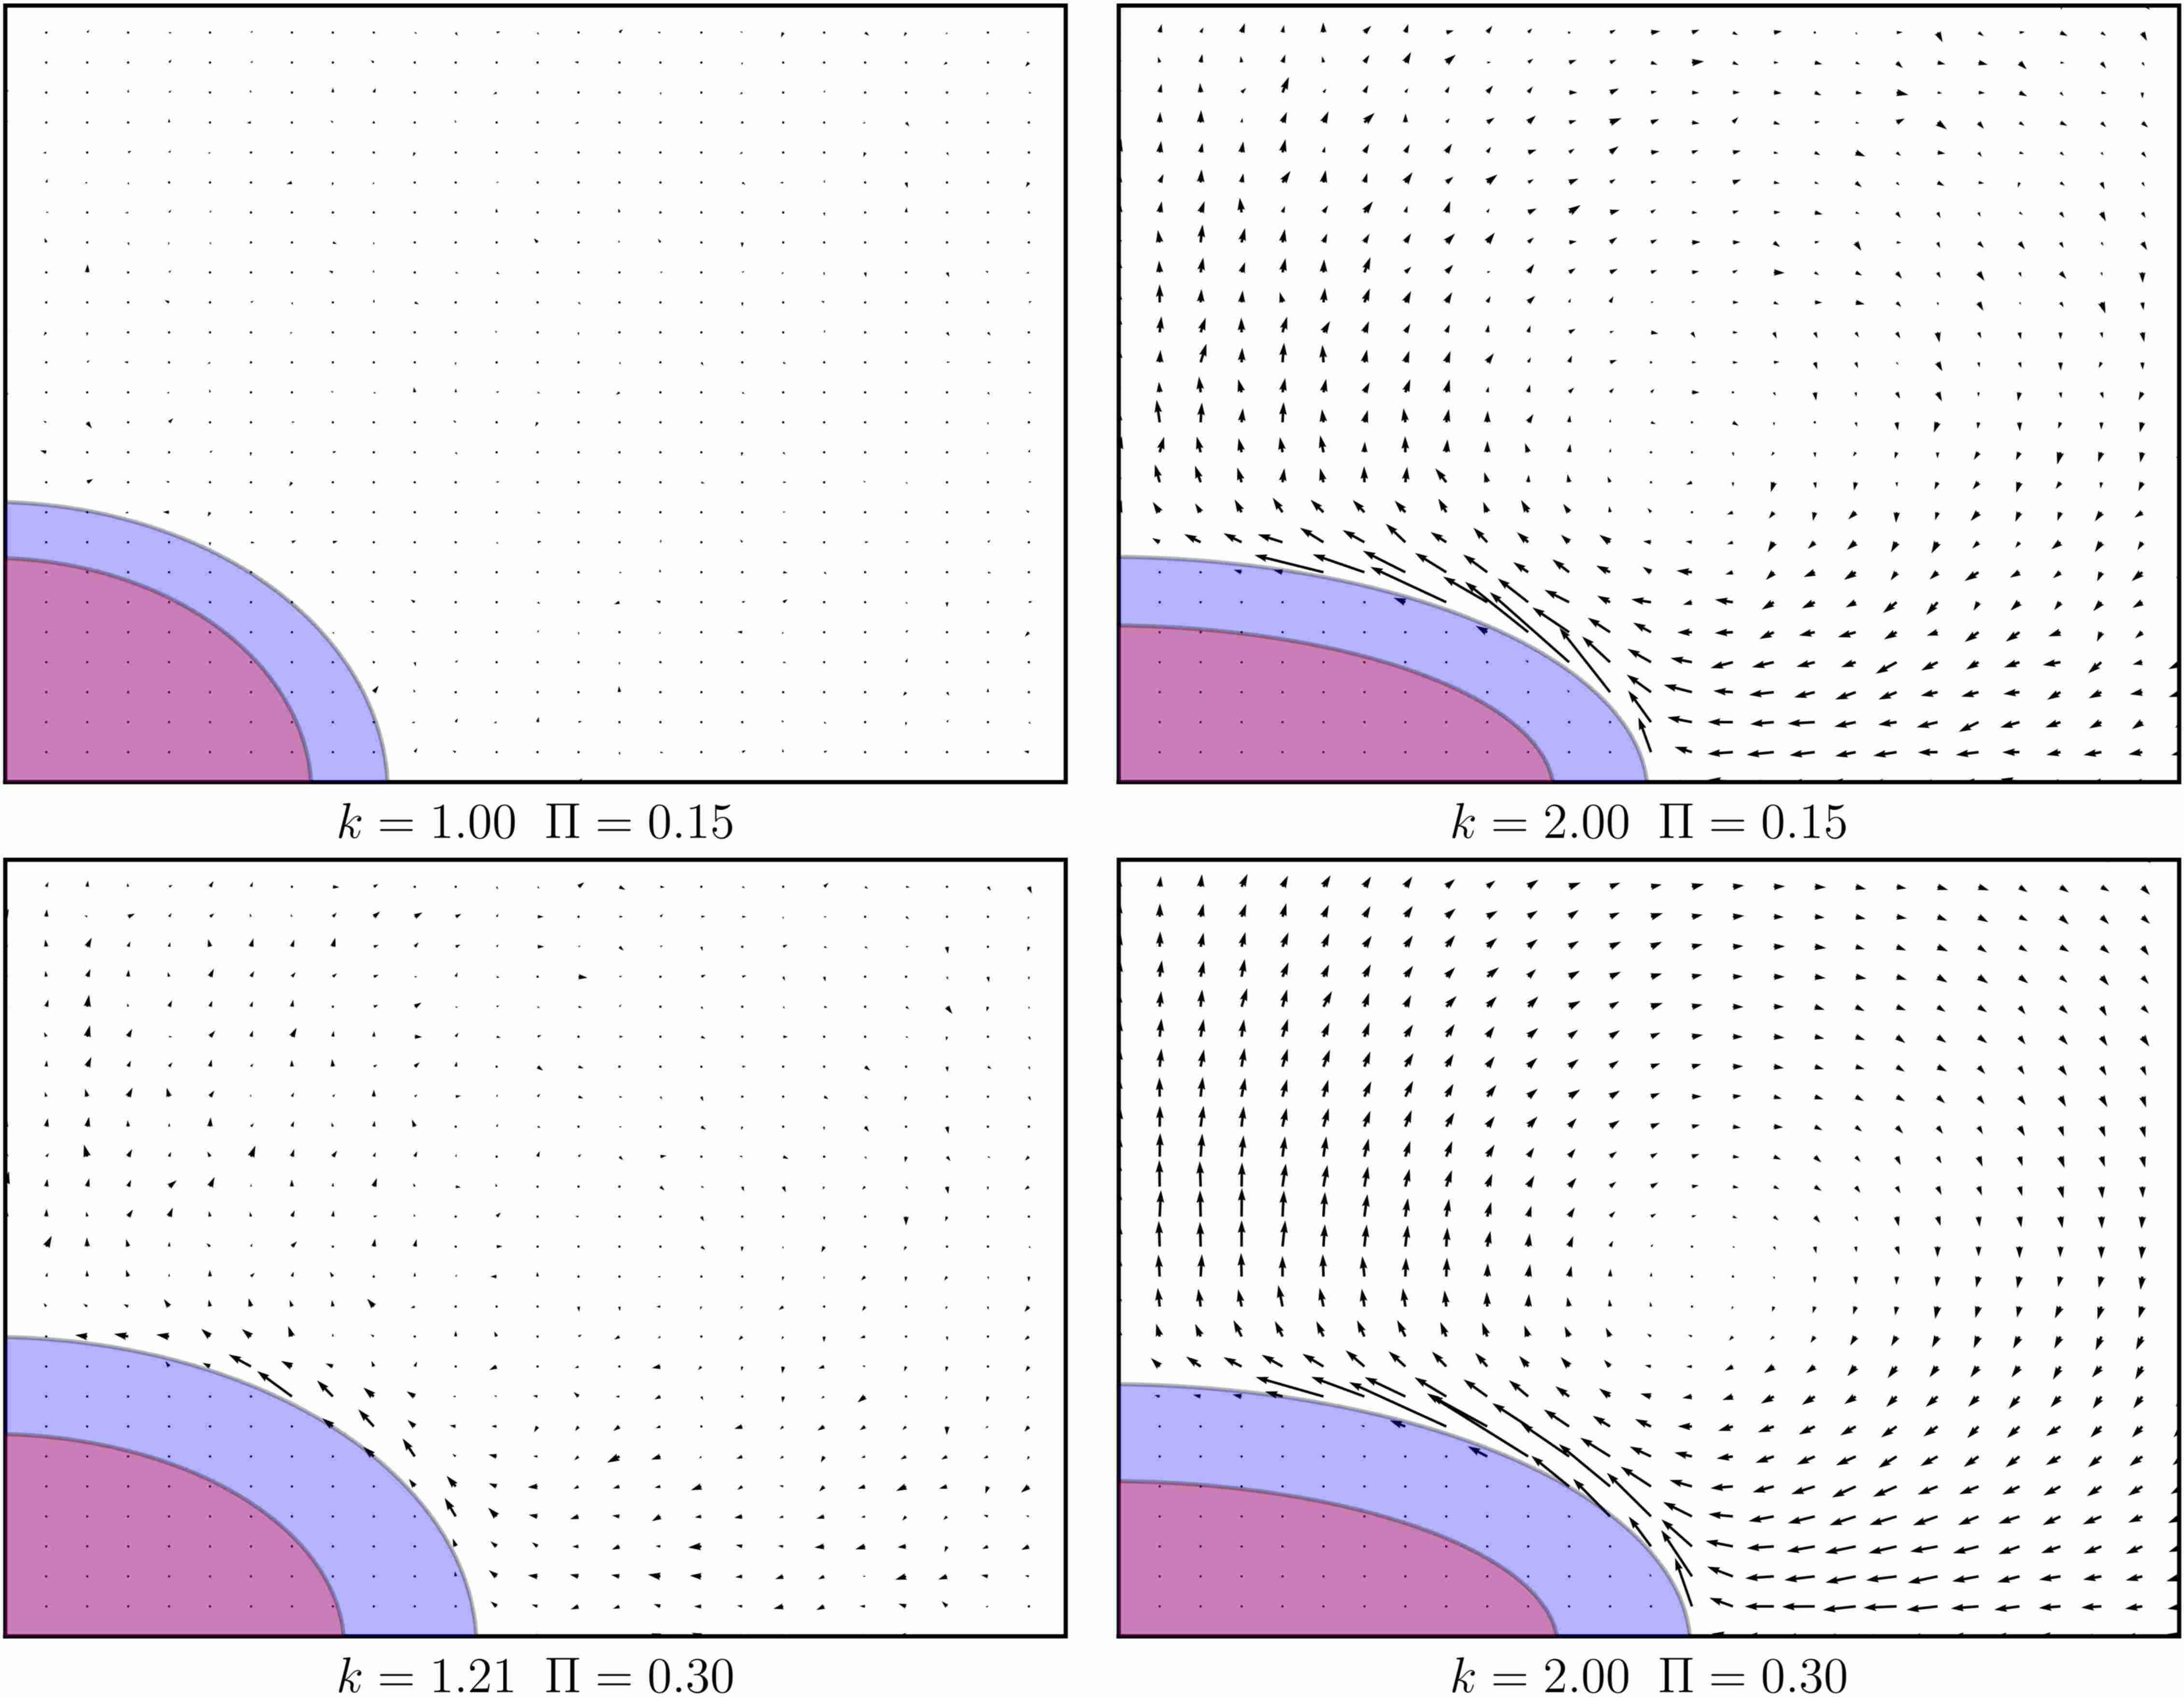
\includegraphics[width=15cm]{entropic_flow_paper/FIG3_fourvelocity.jpg}
\caption{Time-averaged velocity vectors in the upper right quadrant of the simulation for different parameters (shown on chart). For comparison of vector magnitudes the largest arrow in the lower-right graph corresponds to a velocity that is 6.4\% and 11.8\% of the average and median respectively of the initial velocity distribution. The general magnitude of the vectors is highly dependent on the aspect ratio, and disappears completely for a circle ($k=1$). Both the hard-ellipse and an approximation of the depletion zone are shown schematically. }
\label{fig:velocity_plot}
\end{figure}

Motivated by the time-averaged velocity contours which seem to imply a compressing force on the ellipse along the x-axis and an expanding force along the y-axis, an averaged pressure was calculated by recording all momentum changes of the crowder against the ellipse. The average pressure ratio, a heuristic measure designed to measure the tendency of the ellipse to deform, is
%
\begin{equation}
R \equiv \sum_{r,\Delta p \in C}{ \frac{1}{k} \frac{{ \Delta p_x \sgn(r_x) }}{{\Delta p_y \sgn(r_y) } } }
\end{equation}
%
where the sum extends over the set $C$ of all recorded collisions of the crowders against the ellipse, $r,\Delta p$ represent the  position and the change of momentum vectors over the duration of the collision, respectively, with the subscripts indicating the component along the indicated direction, and $\sgn$ is the sign function.

$R$ is a positive function over both increasing aspect ratio and crowder density as show in FIG. \ref{fig:Pratio_plot}. Furthermore it shows the scaling of $R$ is roughly quadratic over an increase of the aspect ratio. Values of $R>1$, more pressure against the major axis, suggest a return to a spherical shape. The results obtained show that the presence of crowders near a fixed aspherical molecule is not the favored state, one that becomes increasingly unfavorable in both crowded conditions and aspect ratio. 

\begin{figure}
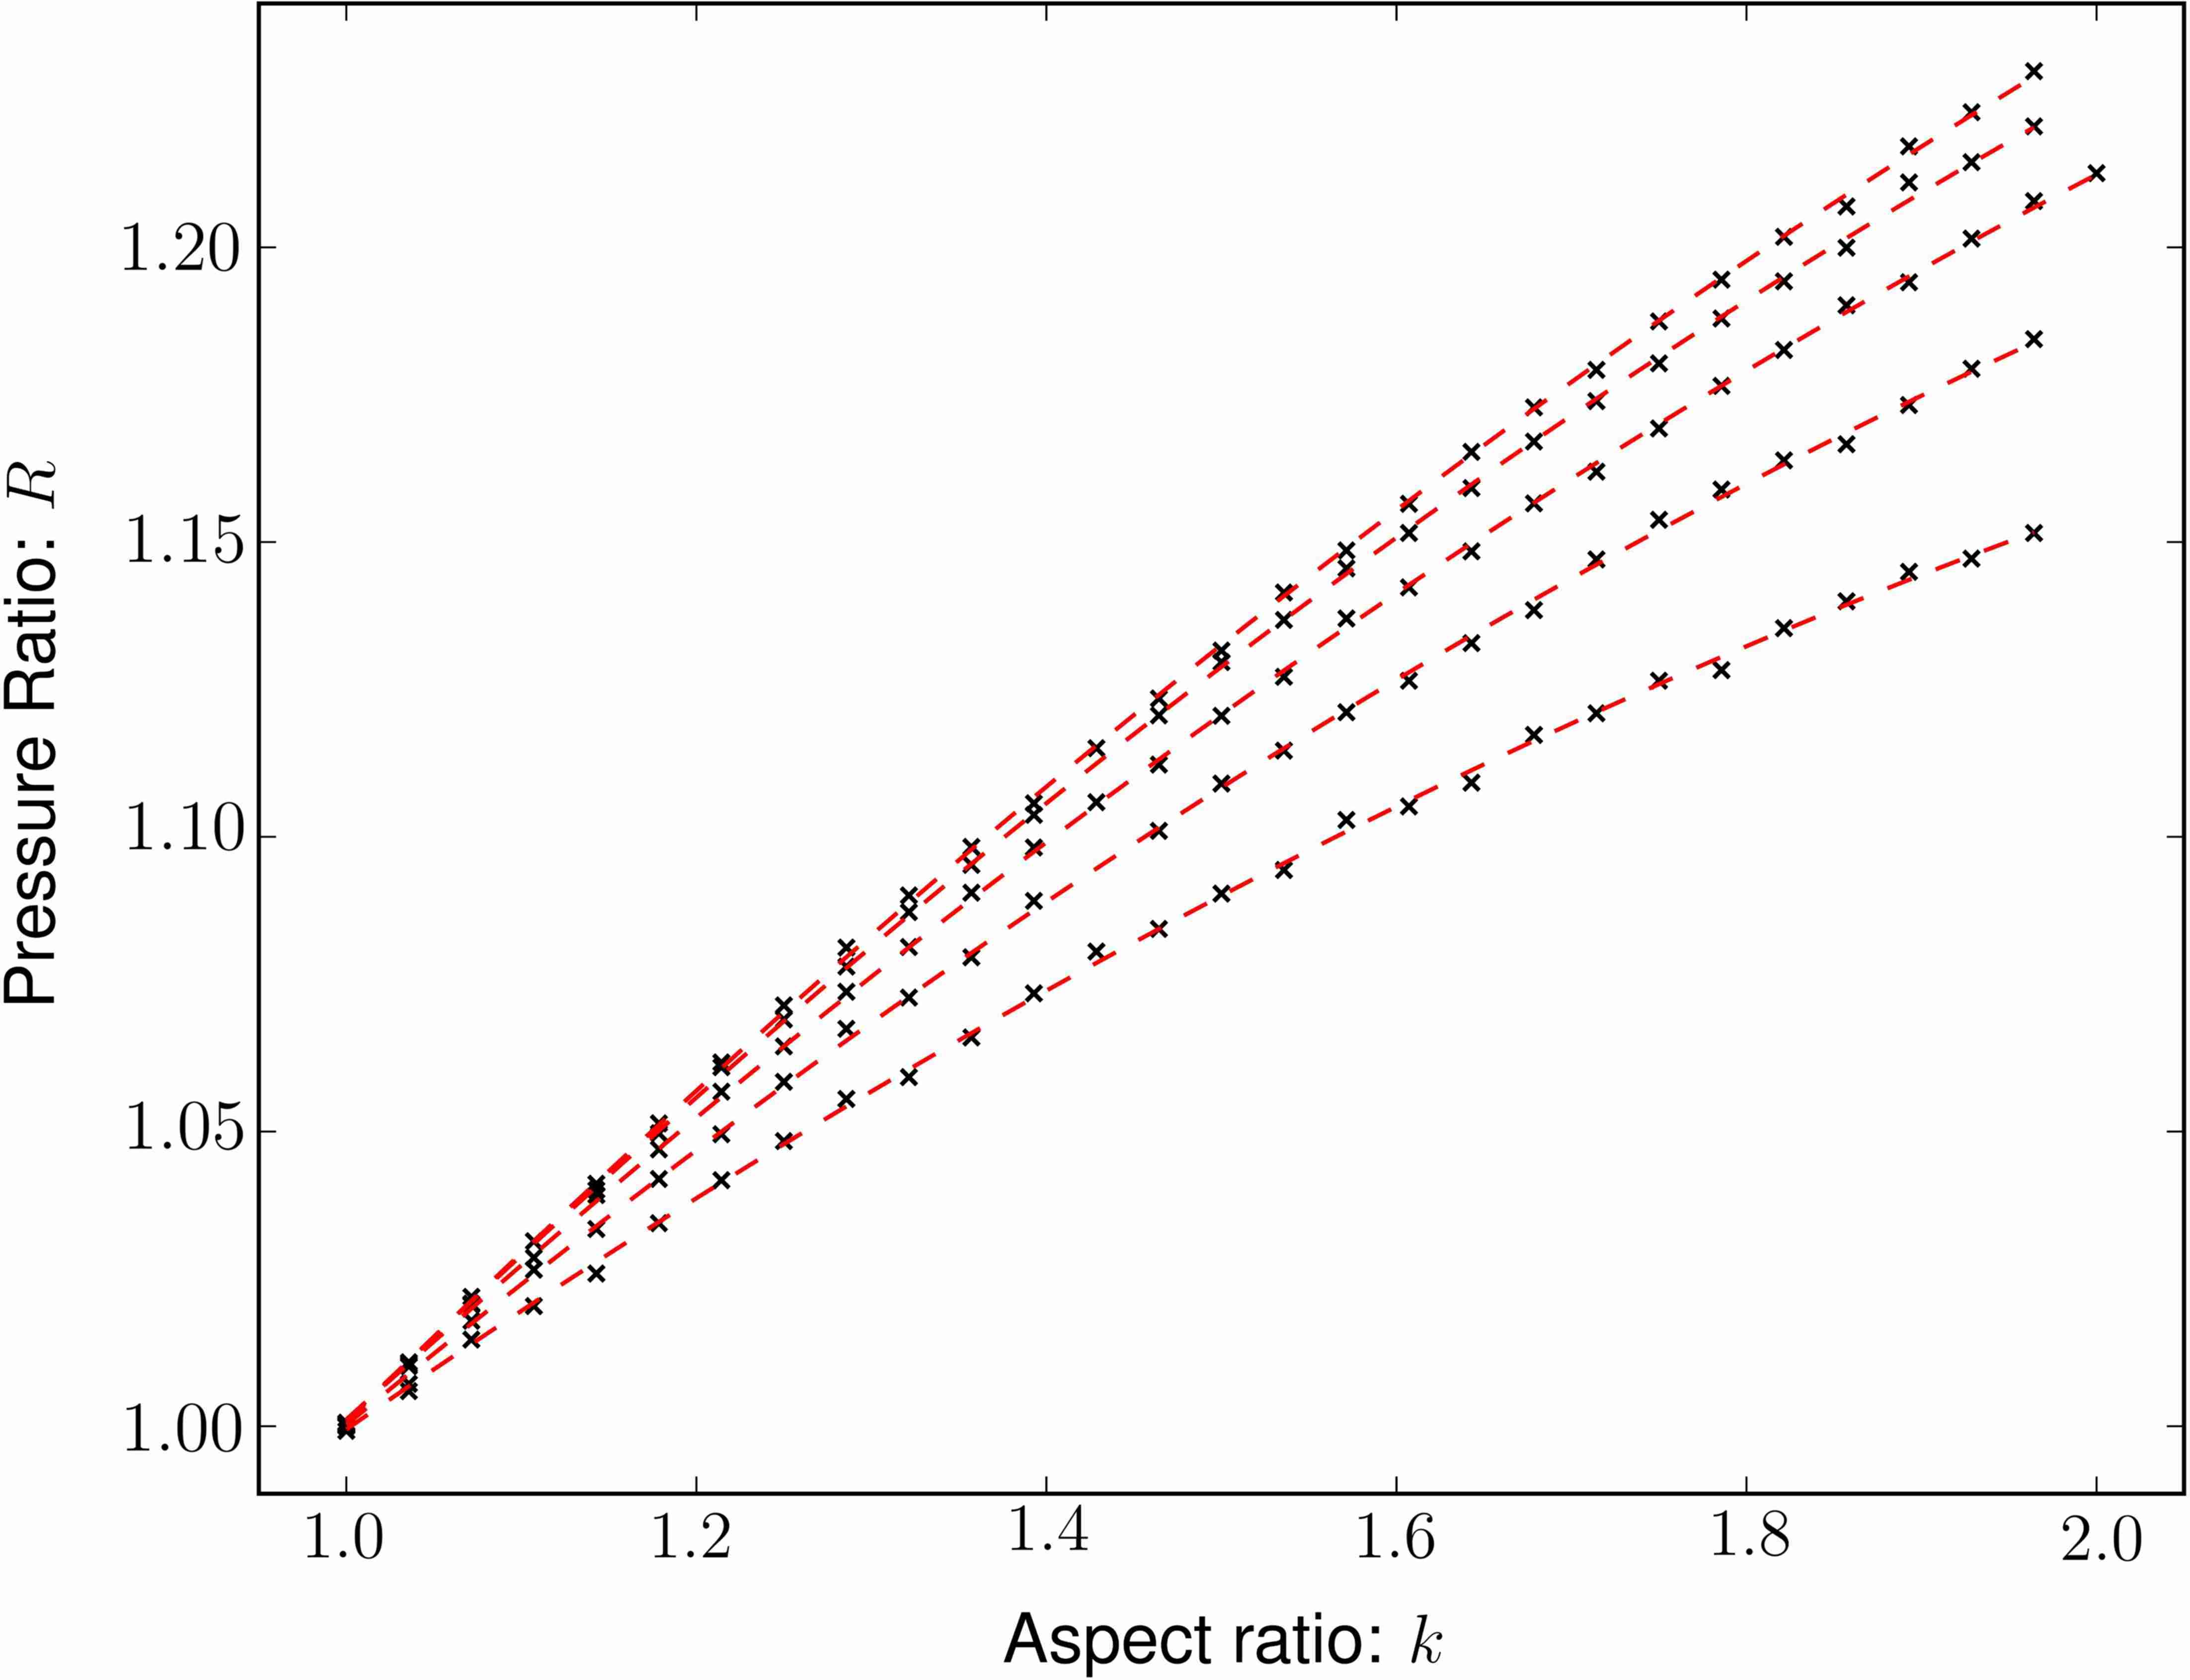
\includegraphics[width=\figurewidthSINGLE]{entropic_flow_paper/FIG4_EDIT.jpg}
\caption{Plot of the pressure ratio $R$ as a function of the aspect ratio $k$ for various values of fixed packing fraction $\Pi$. Each point on the graph represents a complete simulation with different parameters. The values of the fixed packing fraction include $\Pi=[0.10,0.15,0.20,0.25,0.30]$. A quadratic best fit curve shown for each value of $\Pi$ with the bottom curve corresponding to $\Pi=0.10$ and the other curves following sequentially. Note that each curve starts at $R=1.00$ regardless of $\Pi$ since the aspect ratio starts at $k=1.0$. }
\label{fig:Pratio_plot}
\end{figure}

\section{Theoretical Analysis}
As a first approximation, we consider an ideal crowder whose initial distribution is constant at $\rho$ and velocities are drawn from a Boltzmann distribution with temperature $T$. Under a hard-potential the angle of impact at the point of collision along the tangent surface is conserved. When a crowder particle impacts the boundary of the fixed ellipse the resulting trajectory conserves energy but not momentum. We define $\hat N(\phi)$ and $\hat T(\phi)$ to be the normal and tangent unit vectors from the parametrization of the ellipse
%
\begin{align}
\hat N(\phi) = g
\begin{bmatrix}
	E_b \cos \phi \\
	E_a \sin \phi \\
\end{bmatrix}  \\
\hat T(\phi) = g
\begin{bmatrix}
	E_a \sin \phi \\
	-E_b \cos \phi \\
\end{bmatrix}
\end{align}

The incoming and outgoing velocities $\vec v$, $\vec v'$ for are simply
%
\begin{equation}
\vec v' = \vec v - 2 \left ( \vec v \cdot \hat N(\phi) \right ) \hat N(\phi)  
\end{equation}
We can calculate the average angular momentum change for a given $\phi$ by rotating the incident velocity from $0^\circ$ to $180^\circ$ with respect to the tangent. In two dimensions, the cross product of any two vectors $\vec A, \vec B$ becomes a scalar quantity $\ell = \left[ \vec A \times \vec B \right]_{\hat z}=A_x B_y - B_x A_y$. We can define the scalar change of angular momentum with respect to the origin at the point $\vec Q(\phi)$ along the ellipse with incident velocity $\vec v$
%
\begin{align}
& \Delta \ell(\vec v, \phi) = \ell_f - \ell_i = \\
& \left [ \vec Q(\phi) \times \left ( \vec v - 2 \left ( \vec v \cdot \hat N(\phi) \right ) \hat N(\phi) \right ) \right ] _{\hat z} -
\left [\vec Q(\phi) \times \vec v \right ] _{\hat z} \notag
\end{align}

Assuming the crowder is uniformly incident from all angles, the average change in angular momentum at a given point along the ellipse can be found by direct integration of an incoming unit velocity vector
%
\begin{align}
\left < \Delta L(\phi) \right > = &\frac{1}{\pi} \int_0^{\pi} 
{\Delta \ell \left ( R(\theta)\hat T, \phi \right ) d \theta} 
\\
= &\frac{1}{\pi}
\frac
{-2(E_a^2-E_b^2) \cos \phi  \sin \phi }
{\sqrt{E_b^2 \cos^2 \phi - E_a^2 \cos^2 \phi + E_a^2}}
\notag
\end{align}
Where $\theta$ is the incident angle with respect to the tangent point of contact at $\phi$, and $R(\theta)$ is the rotation matrix
%
\begin{equation}
R(\theta) =
\begin{bmatrix} 
\cos \theta && -\sin\theta \\ 
\sin \theta &&  \cos\theta \\  \end{bmatrix}
\end{equation}

Lacking further information on the $\phi$ dependence of the velocity distribution we assume that this distribution is the same at all points. As such, an integration over a range of velocities drawn from a Boltzmann distribution at temperature $T$ would scale the expression by a constant factor. As expected, the expression reduces to $\left < \Delta L(\phi) \right >=0$ for circles. For aspect ratios where $k \neq 1$, we see in FIG. \ref{fig:delta_L} that there are four regions of non-zero $\left < \Delta L(\phi) \right >$ separated by the symmetries of the ellipse. If the crowder particles are allowed to interact, regions of alternating $\left < \Delta L(\phi) \right >$ indicate the potential to develop counter-rotating flows in each quadrant. 
%
\begin{figure}
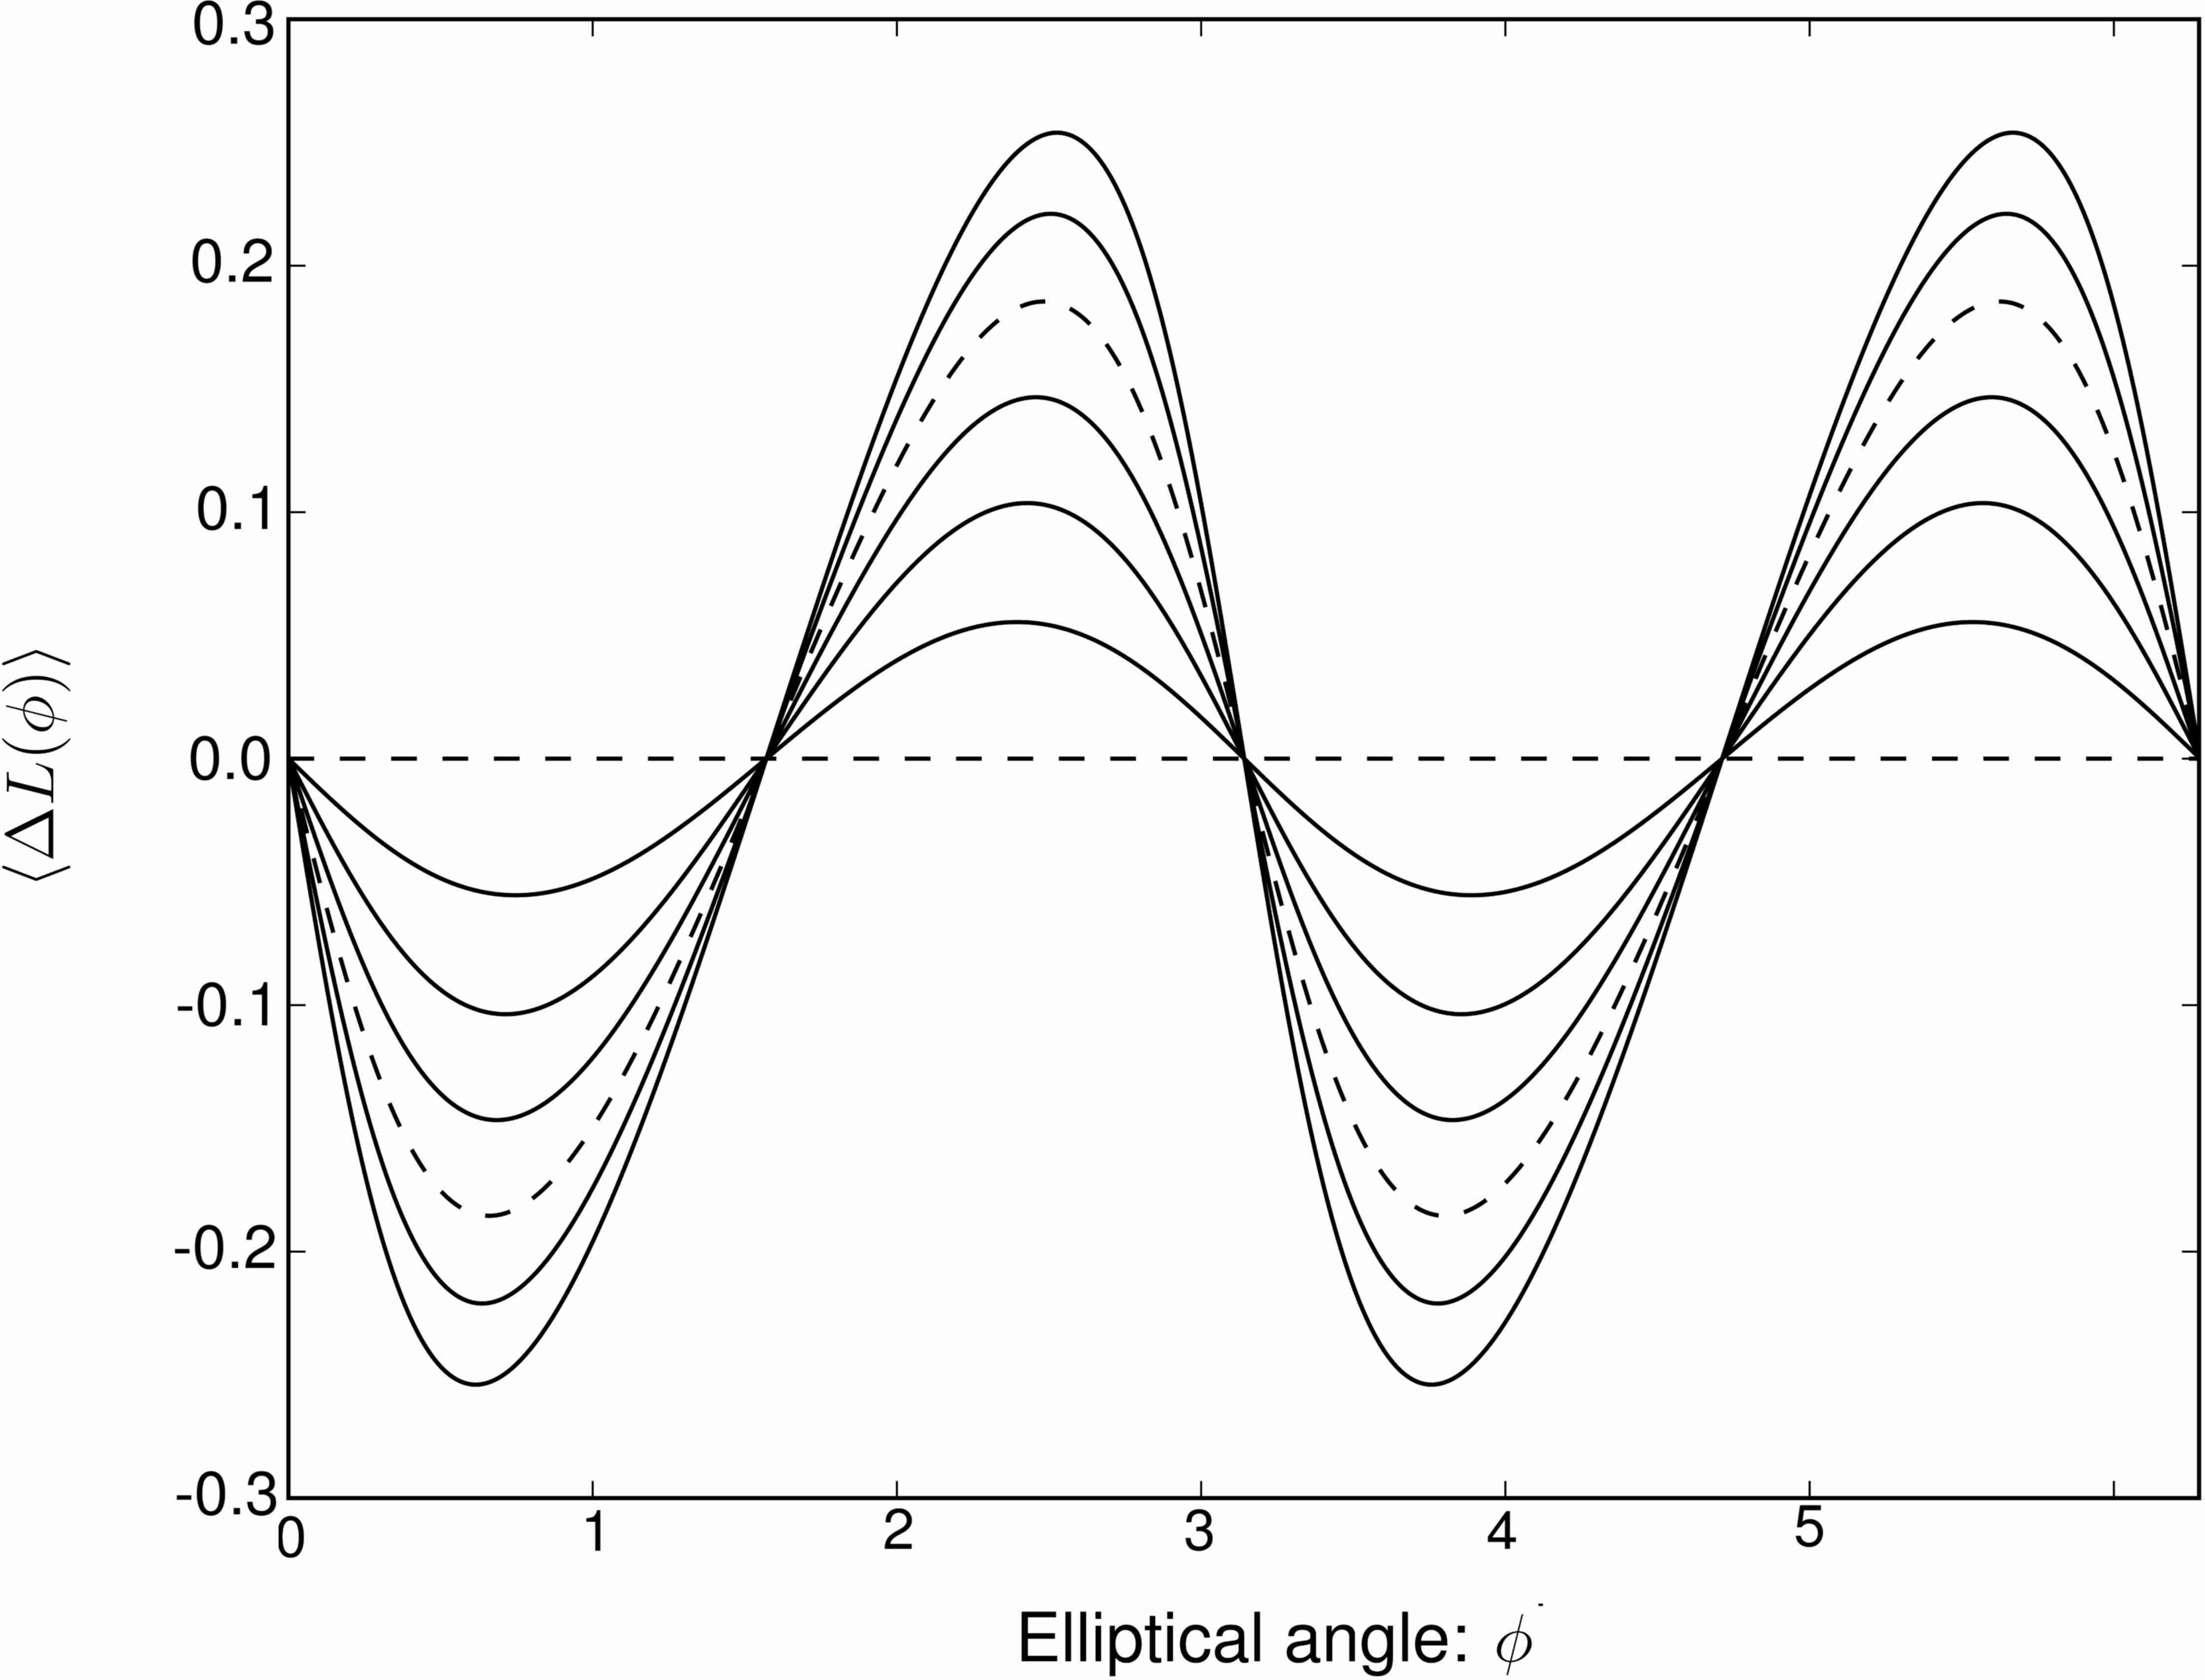
\includegraphics[width=\figurewidthSINGLE]{entropic_flow_paper/FIG5_EDIT.jpg}
\caption{Plot of $\left < \Delta L(\phi) \right >$ for various aspect ratios as a function of the elliptical parameter $\phi$. With area fixed at $E_a E_b \pi=1$, aspect ratios are plotted from $k=E_a/E_b=1$ to $k=2$ in increments of $1/6$. The dashed lines indicate the two curves $k=1,5/3$, with the flat line corresponding to the circle. }
\label{fig:delta_L}
\end{figure}
%
This approximation suffers from several drawbacks; an implicit assumption that the density is constant, that all impact angles $\theta$ have an equal probability, and the point-size radius of the crowders. However, this simplified calculation does suggest the fact that  vortex flow generation and the non-conservation of angular momentum of the system are related.

\section{Discussion}

Molecular dynamics simulations on the microscopic level have long been shown to exhibit behaviors on the macroscopic scale.\cite{rapaport_art_2004} In continuous systems where the flow is obstructed, the non-linear advective term $(\vec v \cdot \nabla) \vec v$ in the Navier-Stokes equation will convert linear momentum into angular momentum.\cite{hannon_molecular_1986} With a high enough Reynolds number, laminar flow around the obstruction becomes unstable and creates pairs of counter-rotating vortices. Theoretical calculations for flow past a sharp-edge plate predict some vortex formation at any non-zero Reynolds number.\cite{miyagi_standing_1983} The fact that vortices exist for any aspect ratio other than unity in our simulation agrees with these results, the difference here is that our system lacks any initial thermal, velocity or density gradients. 

The findings have important implications for all hard-potential models with curvature in the boundary conditions. Related to the original AFM experiment,\cite{yuan_effects_2008} the assumption that the protein has an elliptical shape leads naturally to the questions addressed in our experiment. Namely, does the addition of crowders induce shape changes for a fixed non-spherical molecule? The pressure ratio observed suggested that a return to a spherical shape, one that increased with both ellipticity and packing fraction. This effect is consistent with experimental observations\cite{yuan_effects_2008, homouz_crowded_2008} which show the tendency of macromolecules to return to a spherical shape at progressively higher packing fractions. In the context of the AFM experiment, our simulations agree that the presence of crowders led to a greater unfolding force required.

For the simulations of protein folding and unfolding processes, models of Brownian dynamics are often used. The equivalence of Brownian and hard-disc dynamics has been previously investigated in the literature.\cite{hofling_critical_2008, gleim_relaxation_1998} In a hard-potential simulation all particles maintain an infinite memory of their previous trajectories. Contrast this with the Langevin dynamics which include a viscous damping term along with a random component. In these dynamics the particles maintain only a partial memory of their previous trajectories. In the current simulation, reducing the memory of the particles (by including a viscous drag and random force component) reduces the effect the elliptical boundary condition has on the surrounding environment. In the extreme case of Brownian motion, the density profiles extend only as far as the Brownian steps themselves.  

The point of the above observation is to highlight a crucial difference between hard-sphere simulations with and without memory. The distinction may be irrelevant for a rarefied hard-sphere gas such as argon, but may play a role in the crowded molecular environment. While the role of memory (or lack thereof) in biological simulations is important, we feel that the conclusions drawn from these simulations are still applicable. To the extent that DMD and Brownian dynamics are equivalent, our result can be used to explain both the AFM and shape change experiments.

